\section{What is optimisation?}

An optimisation is one of these words that has many meanings, depending on the context you take as a reference. In the context of this course, optimisation refers to \emph{mathematical optimisation}, which is a discipline of applied mathematics.

In mathematical optimisation, we build upon concepts and techniques from calculus, analysis, linear algebra, and other domains of mathematics to develop methods that allow us finding values for variables within a given domain that maximise (or minimise) the value of a function. In specific, we are trying to solve the following general problem:
%
\begin{align}
    \min &f(x) \label{eq:opt_prob} \\
    \text{s.t.}   &x \in X. \nonumber
\end{align}
%
%where $x \in \reals^n$ is a vector of $n$ \emph{variables}, $f:\mathbb{R}^n \mapsto \reals$ is a \emph{function} to be optimised (minimised) and $X \subseteq \reals^n$ is a \emph{domain} containing acceptable values for $x$.

In a general sense, these problems can be solved by employing the following strategy:
%
\begin{enumerate}
    \item Analysing properties of functions under specific domains and deriving the conditions that must be satisfied such that a point $x$ is a candidate optimal point.
    \item Applying numerical methods that iteratively searches for points satisfying these conditions. 
\end{enumerate}
%
This idea is central in several domains of knowledge, and very often are defined under area-specific nomenclature. Fields such as economics, engineering, statistics, machine learning and, perhaps more broadly, operations research, are intensive users and developers of optimisation theory and applications. 

\subsection{Mathematical programming and optimisation}

Operations research and mathematical optimisation are somewhat intertwined, as they both were born around a similar circumstance. %(Include something on the history of OR)

I like to separate \emph{mathematical programming} from (mathematical) \emph{optimisation}. Mathematical programming is a modelling paradigm, in which we rely on (very powerful, I might add) analogies to model \emph{real-world} problems. In that, we look at a given decision problem considering that
%
\begin{itemize}
    \item \emph{variables} represent \emph{decisions}, as in a business decision or a course of action. Examples include setting the parameter of (e.g., prediction) model, production systems layouts, geometries of structures, topologies of networks, and so forth; 
    \item \emph{domain} represents business rules or \emph{constraints}, representing logic relations, design or engineering limitations, requirements, and such; 
    \item function is an \emph{objective function} that provides a measure of solution quality.  
\end{itemize}
%    
With these in mind, we can represent the decision problem as a \emph{mathematical programming model} of the form of \eqref{eq:opt_prob} that can be solved using \emph{optimisation} methods. From now on, we will refer to this specific class of models as mathematical optimisation models, or optimisation models for short. We will also use the term to \emph{solve the problem} to refer to the task of finding optimal solutions to optimisation models.

This course is mostly focused on the optimisation techniques employed to find optimal solutions for these models. As we will see, depending on the nature of the functions $f$ and $g$ that are used to formulate the model, some methods might be more or less appropriate. Further complicating the issue, for models of a given nature, there might be alternative algorithms that can be employed and with no generalised consense whether one method is generally better performing than another.

\subsection{Types of mathematical optimisation models}

In general, the simpler the assumptions on the parts forming the optimisation model, the more efficient are the methods to solve such problems. 

Let us define some additional notation that we will use from now on. Consider a model in the general form
%
\begin{align*}
	\mini & f(x) \\
	\st   & g_i(x) \leq 0, i = 1, \dots, m \\
	      & h_i(x) = 0, i = 1, \dots, l \\
	      & x \in X,  
\end{align*}
%
where $f: \reals^n \mapsto \reals$ is the objective function, $g:\reals^m \mapsto \reals^m$ is a collection of $m$ inequality constraints and $h: \reals^n \mapsto \reals^l$ is a collection of $l$ equality constraints.

{\bf Remark:} in fact, every inequality constraint can be represented by an equality constraint by making $h_i(x) = g_i(x) + x_{n+1}$ and augmenting the decision variable vector $x \in \reals^n$ to include the slack variable $x_{n+1}$. However, since these constraints are of very different nature, we will explicitly represent both whenever necessary.

The most general types of models are the following. We also use this as an opportunity to define some (admittedly confusing) nomenclature from the field of operations research that we will be using in these notes.
%
\begin{enumerate}
    \item \emph{Unconstrained models:} in these, the set $X = \reals^n$ and $m=l=0$. These are prominent in, e.g., machine learning and statistics applications, where $f$ represents a measure of model fitness or prediction error.  
    \item \emph{Linear programming (LP):} presumes linear objective function. $f(x) = c^\top x$ and constraints $g$ and $h$ affine, i.e., of the form $a_i^\top x - b_i$, with $a_i \in \reals^n$ and $b \in \reals$. Normally, $X = \braces{x \in \reals^n \mid x_j \geq 0, j = 1,\dots, n}$ enforce that decision variables are constrained to be the nonnegative orthant.
    \item \emph{Nonlinear programming (NLP):} some or all of the functions $f$, $g$, and $h$ are nonlinear.
    \item \emph{Mixed-integer (linear) programming (MIP):} consists of an LP in which some (or all) of the variables are constrained to be integers. In other words, $X \subseteq \reals^k \times \integers^{n-k}$. Very frequently, the integer variables are binary terms, i.e., $x_i \in \braces {0,1}$, for $i = 1,\dots, n-k$ and are meant to represent true-or-false or yes-or-no conditions.
    \item \emph{Mixed-integer nonlinear programming (MINLP):} are the intersection of MIPs and NLPs.  
\end{enumerate}

{\bf Remark:} notice that we use the vector notation $c^\top x = \sum_{j \in J} c_j x_j$, with $J = \braces{1,\dots,N}$. This is just a convenience for keeping the notation compact. 


\section{Examples of applications}


We now discuss a few examples to illustrate the nature of the problems to which we will develop solution methods and their applicability to real-world contexts. 

\subsection{Resource allocation and portfolio optimisation} \label{sec:resource_allocation}

In a general sense, any mathematical optimisation model is an instantiation of the \emph{resource allocation problem}. A resource allocation problem consists of how to design an optimal allocation of resources to tasks, such that a given outcome is optimised. 

Classical examples typically include production planning settings, in which raw materials or labour resources are inputted into a system and a collection of products, a production plan, results from this allocation. The objective is to find the best production plan, that is, a plan with the maximum profit or minimum cost. Resource allocation problems can also appear in a less obvious setting, where the resources can be the capacity of transmission lines in an energy generation planning setting, for example.

Let $i \in I = \braces{1,\dots, M}$ be a collection of resources and $j \in J = \braces{1,\dots,N}$ be a collection of products. Suppose that, to produce one unit of product $j$, a quantity $a_{ij}$ of resource $i$ is required. Assume that the total availability of resource $i$ is $b_i$ and that the return per unit of product $j$ is $c_j$.

Let $x_j$ be the decision variable representing total of product $j$ produced. The resource allocation problem can be modelled as
%
\begin{align}
	\maxi \ & \sum_{j \in J} c_j x_j \label{ex1:obj} \\
	\st & \sum_{j \in J}a_{ij} x_j \leq b_i, \ \forall i \in I \label{ex1:const1} \\
	& x_j \geq 0, \ \forall j \in J. \label{ex1:const2}
\end{align} 
%
Equation \eqref{ex1:obj} represents the objective function, in which we maximise the total return obtained from a given production plan. Equation \eqref{ex1:const1} quantify the resource requirements for a given production plan and enforce that such a requirement does not exceed the resource availability. Finally, constraint \eqref{ex1:const2} defines the domain of the decision variables.

Notice that, as posed, the resource allocation problem is linear. This is perhaps the most basic, and also most diffused setting for optimisation models for which very reliable and mature technology is available. In this course, we will concentrate on methods that can solve variants of this model in which the objective function and/or the constraints are required to include nonlinear terms. 

One classic variant of resource allocation that include nonlinear terms is the \emph{portfolio optimisation problem}. In this, we assume that a collection of assets $j \in J = \braces{1,\dots, N}$ are available for investment. In this case, capital is the single (actual) resource to be considered. Each asset has random return $R_j$, with an expected value $\mathbb{E}[R_j] = \mu_j$. Also, the covariance between two assets $i,j \in J$ is given by $\sigma_{ij} = \mathbb{E}[(R_i - \mu_i)(R_j - \mu_j)]$, which can be denoted as the covariance matrix 
%
\begin{align*}
	\Sigma = \begin{bmatrix}
		\sigma_{11} & \dots & \sigma_{1N} \\ 
		\vdots      & \ddots & \vdots \\
		\sigma_{N1}  & \dots & \sigma_{NN}
	\end{bmatrix}
\end{align*}
%
Markowitz (1952) proposed using $x^\top\Sigma x$ as a risk measure that captures the variability in the return of the assets. Given the above, the optimisation model that provides the investment portfolio with the least risk, given a minimum requirement $\epsilon$ in terms of expected returns is given by
%
\begin{align}
	\mini \ &  x^\top\Sigma x \label{ex2:obj} \\
	\st & \mu^\top x  \geq \epsilon \label{ex2:const1}\\
	& 0 \leq x_j \leq 1, \ \forall j \in J. \label{ex2:const2}
\end{align} 
%
Objective function \eqref{ex2:obj} represents the portfolio risk to be minimised, while constraint \eqref{ex2:const1} enforces that the expected return must be at least $\epsilon$. Notice that $\epsilon$ can be seen as a resource that has to be (at least) completely depleted, if one wants to do a parallel with the resource allocation structure discussed early. Constraint \eqref{ex2:const2} defined the domain of the decision variables. Notice how the problem is posed in a scaled form, where $x_j \in [0,1]$ represents a percentage of a hypothetical available capital for investment.

In this example, the problem is nonlinear due to the quadratic nature of the objective function $x^\top\Sigma x = \sum_{i,j \in J} \sigma_{ij}x_ix_j$. As we will see later on, there are efficient methods that can be employed to solve quadratic problems like this.


\subsection{The pooling problem: refinery operations planning}

The \emph{pooling problem} is another example of a resource allocation problem that naturally presents nonlinear constraints. In this case, the production depends on \emph{mixing operations}, known as pooling, to obtain certain product specification for a given property.

As an illustration, suppose that products $j \in J = \braces{1,\dots,N}$ are produced by mixing byproducts $i \in I_j \subseteq I = \braces{1,\dots,M}$. Assume that the qualities of byproducts $q_i$ are known and that there is no reaction between byproducts. Each product is required to have a property value $q_j$ within an acceptable range $[\underline{q}_j, \overline{q}_j]$ to be classified as product $j$. In this case, mass and property balances are calculated as
%
\begin{align}
	& x_j  = \sum_{i \in I_j}{x_i}, \ \forall j \in J \\
	& q_j = \frac{\sum_{i \in I_j}q_ix_i}{x_j}, \ \forall j \in J \label{ex3:const2}.
\end{align}
%
These can then incorporated into the resource allocation problem accordingly. One key aspect associated with pooling problem formulations is that the property balances represented by \eqref{ex3:const2} define \emph{nonconvex} feasibility regions. As we will see later, convexity is a powerful property that allows for developing efficient solution methods and its absence typically compromises computational performance and tractability in general.

  
\subsection{Robust optimisation}

Robust optimisation is a subarea of mathematical programming concerned with models that support decision-making under \emph{uncertainty}. In specific, the idea is to devise a formulation mechanism that can guarantee feasibility of the optimal solution in face of variability, ultimately taking a risk-averse standpoint. 

Consider the resource allocation problem from Section \ref{sec:resource_allocation}. Now, suppose that the parameters $\tilde{a}_i \in \reals^N $ associated with a given constraint $i \in I = \braces{1,\dots,M}$ are uncertain with a unknown probability distribution. The resource allocation problem can then be formulated as
%
\begin{align*}
	\maxi \ &  c^\top x  \\
	\st & \tilde{a}_{i}^\top x \leq b_i, \ \forall i \in I  \\
	& x_j \geq 0, \ \forall j \in J. 
\end{align*} 
%
Let us assume that the only information available are observations $\hat{a}_i$, from which we can estimate a nominal value $\overline{a}_i$. This is illustrated in Figure \ref{fig:random_observations}, in which 100 random observations are generated for $\tilde{a_i} = [\tilde{a}_{i1}, \tilde{a}_{i2}]$ with $\tilde{a}_{i1} \sim \text{Normal}(10,2)$ and $\tilde{a}_{i2} \sim \text{Normal}(5,3)$ for a single constraint $i \in I$. The nominal values are assumed to have coordinates given by the average values used in the Normal distributions. 
%
\begin{figure}[h]
	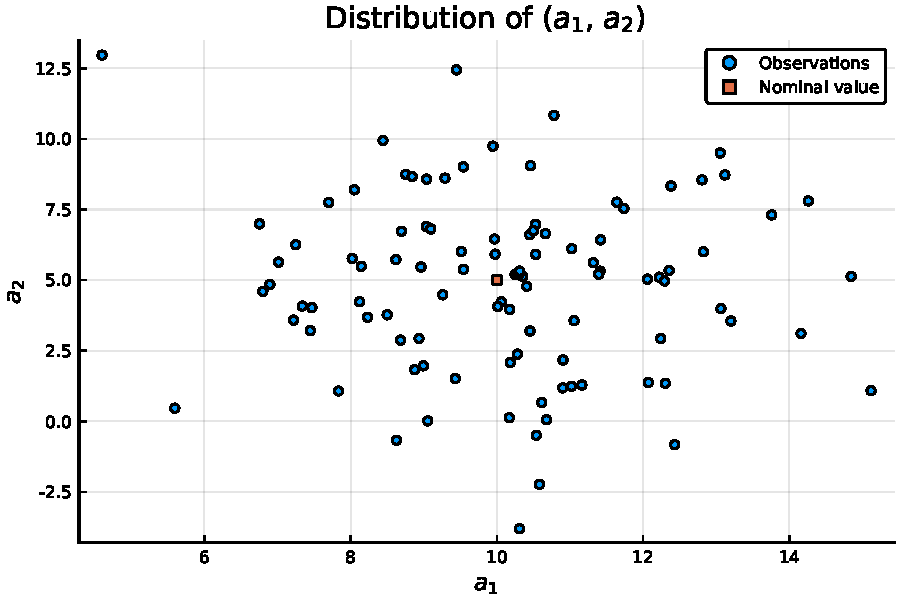
\includegraphics[width=0.8\textwidth]{part_2/chapter_1/figures/data_no_ellipsoid.pdf}
	\caption{One hundred random realisations for $\tilde{a}_i$.} \label{fig:random_observations}
\end{figure}
%
Our objective is to develop a model that incorporates a given level of protection in terms of feasibility guarantees. That is, we would like to develop a model that provides solutions that are guaranteed to remain feasible if the realisation of $\tilde{a}_i$ falls within an \emph{uncertainty set} $\epsilon_i$ of size controlled by the parameter $\Gamma_i$. The idea is that the bigger the uncertainty set $\epsilon_i$, the more robust is the solution, which typically comes at the expense of accepting solutions with expected worse performance.

The tractability of robust optimisation models depends on the geometry of the uncertainty set employed. Let us assume in what follows that 
%
\begin{align}
	\epsilon_i = \braces{\overline{a}_i + P_iu \mid ||u||_2 \leq \Gamma_i} \label{eq:ellipsoid}
\end{align}
%
is an ellipsoid with the characteristic matrix $P_i$ (i.e., its eigenvalues show how the ellipsoid extends in every direction from $\overline{a}_i$) and $\Gamma_i$ employs a scaling of the ellipsoid size.

{\bf Remark:} an alternative (perhaps more frequent) characterisation of an ellipsoid $\epsilon \subset \reals^n$ centred at $\overline{x}$ is given by $\epsilon = \braces{x \in \reals^n \mid (x - \overline{x})^\top A(x - \overline{x}) = 1}$. By making $A = P^{-2}$, we recover the representation in \eqref{eq:ellipsoid}.

We can now formulate the \emph{robust counterpart}, which consists of a risk-averse version of the original resource allocation problem. In that, we try to anticipate the worst possible outcome and make decisions that are both optimal and guarantee feasibility in this worst-case sense. This standpoint translates into the following optimisation model.
%
\begin{align}
	\maxi \ &  c^\top x \nonumber \\
	\st & \maxi_{a_{i} \in \epsilon_i}\braces{a_i^\top x} \leq b_i, \ \forall i \in I \label{ex3:robust_const}\\
	& x_j \geq 0, \forall j \in J. \nonumber
\end{align}
%
Notice how the constraint \eqref{ex3:robust_const} has an embedded optimisation problem, turning into a \emph{bi-level optimisation} problem. This highlights the issue associated with tractability, since solving the whole problem strongly depends on deriving tractable equivalent reformulations.

Assuming that the uncertainty set $\epsilon_i$ is an ellipsoid, the following result holds.
%
\begin{align}
	\max_{a_{i} \in \epsilon_i}\braces{a_i^\top x}  & = \overline{a}_i^\top x + \max_u\braces{u^\top P_i x : ||u||_2 \leq \Gamma_i} \label{eq:robust_set1}\\
	& = \overline{a}_i^\top x + \Gamma_i||P_i x||_2. \label{eq:robust_set2}
\end{align}
%
In \eqref{eq:robust_set1}, we recast the inner problem in terms of the ellipsoidal uncertainty set, ultimately meaning that we recast the inner maximisation problem in terms of variable $u$. Since the only constraint is $||u||_2 \leq \Gamma_i$, in \eqref{eq:robust_set2} we can derive a closed form for the inner optimisation problem.

With the closed form derived in \eqref{eq:robust_set2}, we can reformulate the original bi-level problem as a tractable single-level problem of the following form
%
\begin{align}
	\maxi \ &  c^\top x \nonumber \\
	\st & \overline{a}_i^\top x + \Gamma_i||P_i x||_2 \leq b_i, \ \forall i \in I \label{eq:robust_counter1}\\
	& x_j \geq 0, \ \forall j \in J. \nonumber
\end{align} 
%
Notice how the term $\Gamma_i||P_i^\top x||_2$ creates a buffer for constraint \eqref{eq:robust_counter1}, ultimately preventing the complete depletion of the resource. Clearly, this will lead to a suboptimal solution when compared to the original deterministic at the expense of providing protection against deviations in coefficients $a_i$. This difference is often referred to as the \emph{price of robustness}.

In Figure \ref{fig:ellipsoids}, we show the ellipsoidal sets for two levels of $\Gamma_i$ for a single constraint $i$. We define 
%
\begin{align}
	\epsilon_i = \braces{\begin{bmatrix} 10 \\ 5 \end{bmatrix} + \begin{bmatrix} 2 & 0 \\ 0 & 3 \end{bmatrix} \begin{bmatrix} u_1 \\ u_2 \end{bmatrix}}
\end{align}
%
using the average and standard deviation of the original distributions that generated the observations. We plot the ellipsoids for $\Gamma_1 = 1$ and $\Gamma_2 = 1.5$, illustrating how the protection level increases as $\Gamma$ increases. This can be inferred since the uncertainty set covers more of the observations and the formulation is such that feasibility is guaranteed for any observation within the uncertainty set. 
%
\begin{figure}
	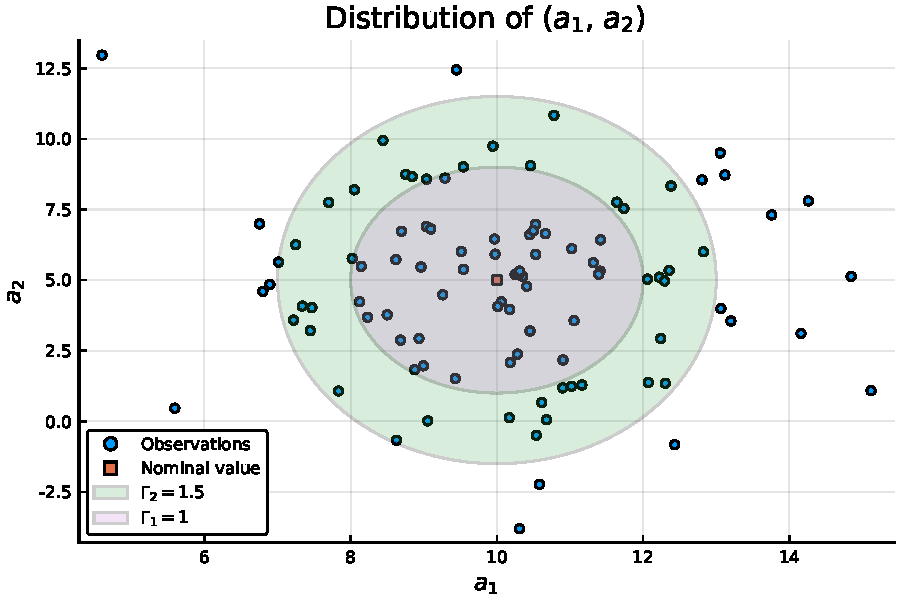
\includegraphics[width=0.8\textwidth]{part_2/chapter_1/figures/data_with_ellipsoid.pdf}
	\caption{One hundred random realisations for $\tilde{a}_i$.} \label{fig:ellipsoids}
\end{figure}
%


\subsection{Classification: support-vector machines}

This is an example in which the resource allocation structure within the optimisation model is not as obvious. Suppose we are given a data set $D \in \reals^{n}$ with $|D| = N + M$ that can be divided into two disjunct sets $I^- = \braces{x_1, \dots, x_N}$ and $I^+ = \braces{x_1,\dots, x_M}$. 

Each element in $D$ is an observation of a given set of $n$ features with values represented by a $x \in \reals^n$ that has been classified as belonging to set $I^-$ and $I^+$. Because of the availability of labelled data, classification is said to be ane xample of supervised learning in the field of machine learning. 

Figure \ref{fig:classified_observations} illustrates this situation for $n = 2$, in which the orange dots represent points classified as belonging to $I^-$ (negative observations) and the blue dots represent points classified as belonging to $I^+$ (positive observations).

\begin{figure}
    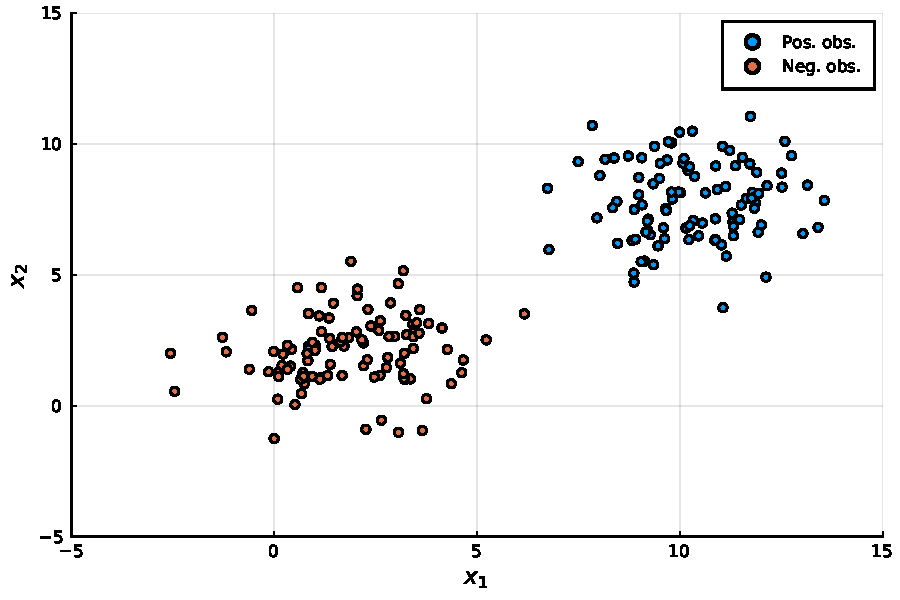
\includegraphics[width=0.8\textwidth]{part_2/chapter_1/figures/classes_no_classifier.pdf}
    \caption{Two hundred observations for $x_i$ classified to belong to $I^-$ (orange) or $I^+$ (blue).}        
    \label{fig:classified_observations}
\end{figure}

Our task is to obtain a function $f:\reals^n \mapsto \reals$ from a given family of functions that is capable to, given an observed set of features $\hat{x}$, classify whether it belongs to $I^-$ or $I^+$. In other words, we want to calibrate $f$ such that
%
\begin{align}
	f(x_i) < 0, \ \forall x_i \in I^-, \text{ and } f(x_i) > 0, \ \forall x_i \in I^+.  
\end{align}
%
This function would then act as a classifier that could be employed to any new observation $\hat{x}$ made. If $f$ is presumed to be an affine function of the form $f(x) = a^\top x - b$, then we obtain a \emph{linear classifier}. 

Our objective is to obtain $a \in \reals^n$ and $b \in \reals$ such that misclassification error is minimised. Let us define the error measure as
%
\begin{align*}
& e^-(x_i \in I^-; a, b) := 
    \begin{cases} 0, \text{ if } a^\top x_i - b \leq 0, \\
        a^\top x_i - b, \text{ if } a^\top x_i - b > 0.
    \end{cases} \\
& e^+(x_i \in I^+; a, b) := 
    \begin{cases} 0, \text{ if } a^\top x_i - b \geq 0, \\
        b -  a^\top x_i, \text{ if } a^\top x_i - b < 0.
    \end{cases}                   
\end{align*}
%
Using this error measure, we can define constraints that capture deviation on each measure by means of nonnegative slack variables. Let $u_i \geq 0$ for $i = 1, \dots, N$ and $v_i \geq 0$ for $i = 1,\dots, M$ be slack variables that measure the \emph{misclassification error} for $x_i \in I^-$ and $x_i \in I^+$, respectively.

The optimisation problem that finds optimal parameters $a$ and $b$ can be stated as
%
\begin{align}
	\mini \ & \sum_{i=1}^M u_i + \sum_{i=1}^N v_i \label{ex4:obj}\\
	\st & a^\top x_i - b - u_i \leq 0, i = 1, \dots, M \label{ex4:const1} \\
    & a^\top x_i - b + v_i \geq 0, i = 1,\dots,N \label{ex4:const2} \\
    & ||a||_2 = 1 \label{ex4:const3} \\
    & u_i \geq 0, i = 1, \dots, N \\
    & v_i \geq 0, i = 1, \dots, M \\
    & a \in \reals^n, b \in \reals. \label{ex4:end}   
\end{align} 
%
The objective function \eqref{ex4:obj} accumulates the total misclassification error. Constraint \eqref{ex4:const1} allows for capturing the misclassification error for each $x_i \in I^-$. Notice that $u_i = \max\braces{0, a^\top x_i -b} = e^-(x_i \in I^-; a, b)$. Likewise, constraint \eqref{ex4:const2} guarantees that $v_i = e^+(x_i \in I^+; a, b)$.
To avoid trivial solutions in which $(a,b) = (0, 0)$, the normalisation constraint $|| a ||_2 = 1$ is imposed in constraint \eqref{ex4:const3}, which turns the model nonlinear.

Solving the model \eqref{ex4:obj}--\eqref{ex4:end} provides optimal $(a,b)$ which translates into the classifier represented as the green line in Figure \ref{fig:observations_with_classifier}.

\begin{figure}[h]
    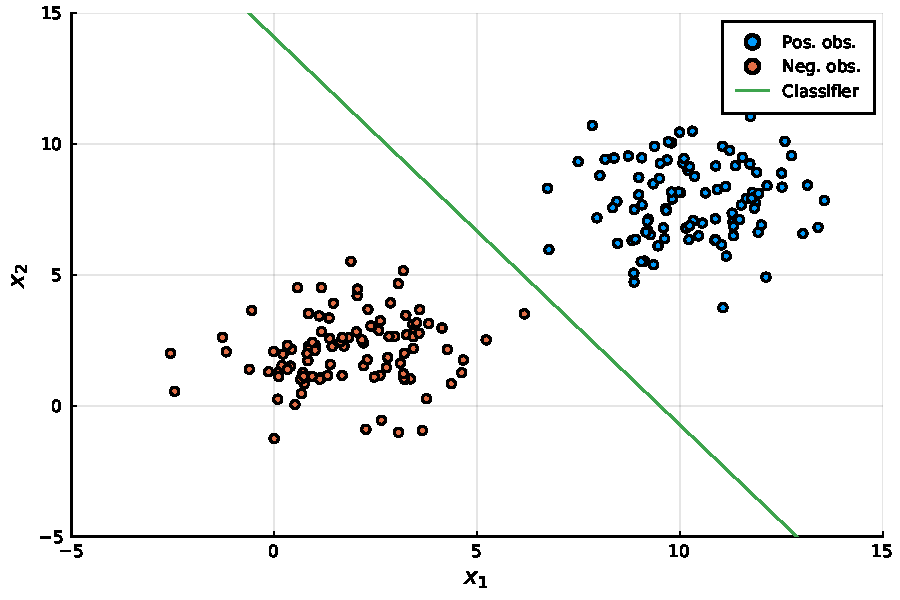
\includegraphics[width=0.8\textwidth]{part_2/chapter_1/figures/classes_with_classifier.pdf}
    \caption{Two hundred observations for $x_i$ classified to belong to $I^-$ (orange) or $I^+$ (blue) with a classifier (green).}        
    \label{fig:observations_with_classifier}
\end{figure}
 
A variant referred to as \emph{robust classifier} penalises not only the the misclassification error, but also the observations within a given slab $S = \braces{x \in \reals^n \mid -1 \leq a^\top x - b \leq 1}$. Notice that, being the two lines defined by $f^-(x) : a^\top x - b = -1$ and $f^+(x) : a^\top x - b = +1$, the distance between the two hyperplanes is given by $\frac{2}{||a||_2}$. 

Accordingly, we redefine our error measures as follows. 
%
\begin{align*}
	& e^-(x_i \in I^-; a, b) := 
	    \begin{cases} 0, \text{ if } a^\top x_i - b \leq -1, \\
	        |a^\top x_i - b|, \text{ if } a^\top x_i - b > -1.
	    \end{cases} \\
	& e^+(x_i \in I^+; a, b) := 
	    \begin{cases} 0, \text{ if } a^\top x_i - b \geq 1, \\
	        |b -  a^\top x_i|, \text{ if } a^\top x_i - b < 1.
	    \end{cases}                   
\end{align*}
%
By doing so, a penalty is applied not only to those points that were misclassified but also to those points correctly classified that happen to be inside the slab $S$. To define an optimal robust classifier, one must trade off the size of the slab, which is inversely proportional to $||a||$, and the total of observations that fall in the slab $S$. The formulation for the robust classifier then becomes
%
\begin{align}
	\mini \ & \sum_{i=1}^M u_i + \sum_{i=1}^N v_i + \gamma||a||_2^2 \label{ex5:obj}\\
	\st & a^\top x_i - b - u_i \leq -1, \ i = 1,\dots,M \label{ex5:const1} \\
	    & a^\top x_i - b + v_i \geq 1, \ i = 1,\dots,N \label{ex5:const2} \\
	    & u_i \geq 0, i = 1, \dots, N \\
	    & v_i \geq 0, i = 1, \dots, M \\
	    & a \in \reals^n, b \in \reals.
\end{align} 
%  
In objective function \eqref{ex5:obj}, the errors accumulated in variables $u_i$, $i=1,\dots,N$ and $v_i$, $i = 1,\dots,M$ and the squared norm $||a||_2^2$ are considered simultaneously. The term $\gamma$ is a scalar used to impose an emphasis on minimising the norm $||a||_2$ and incentivising a larger slab $S$ (recall that the slab is large for smaller $||a||_2$). The squared norm  $||a||_2^2$ is considered instead as a means to recover differentiability, as the norm  $||a||_2$ is not differentiable. Later on, we will see how beneficial it is for optimisation methods to be able to assume differentiability. Moreover, note how in constraints \eqref{ex5:const1} and \eqref{ex5:const2} $u$ and $v$ also accumulate penalties for correctly classified $x_i$ that happen to be between the slab $S$, that is, that have term $a^\top x - b$ larger/ smaller than -1/ +1. Figure \ref{fig:observations_with_rob_classifier} shows a robust classifier an arbitrary value of $\gamma$.

\begin{figure}[H]
    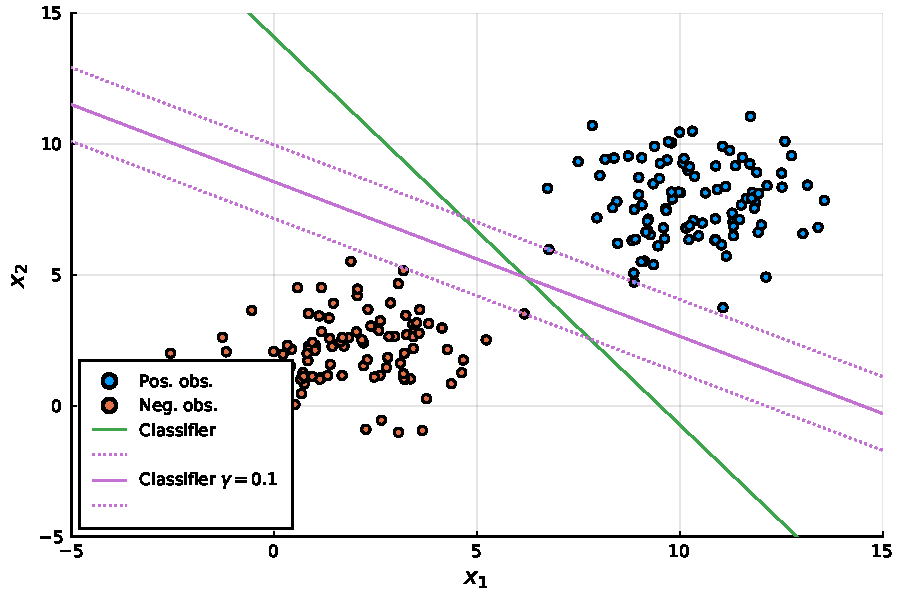
\includegraphics[width=0.8\textwidth]{part_2/chapter_1/figures/classes_with_robust_classifier.pdf}
    \caption{Two hundred observations for $x_i$ classified to belong to $I^-$ (orange) or $I^+$ (blue).}        
    \label{fig:observations_with_rob_classifier}
\end{figure}


{\bf Remark:} robust classifiers are known in the machine learning literature as \emph{support vector machines}, where the support vectors are the observations that support the slab. 
